\documentclass[a4paper, czech]{article}

\title{Úloha č.1: Efekt Fuzz Face – Simulace a měření}
\author{Karolína Andrea Šebestová}
\date{Datum měření: 24.9.2024}

\usepackage[czech]{babel}
\usepackage{indentfirst}
\usepackage{graphicx}
\usepackage{float}
\usepackage[margin=1.5cm]{geometry}
\usepackage{booktabs}
\usepackage{amsmath}

\begin{document}

\maketitle


\begin{figure}[H]
    \centering
    
\includegraphics{fuzz_face_schema.png}
    % \caption{Zapojení diody v propustném a v závěrném směru}
\end{figure}

\section{Úkoly měření}

\begin{enumerate}
    \item Na počítači spusťte soubor D:\textbackslash NKZT\textbackslash LTspice\textbackslash Fuzz\_face\_trans.asc, který se otevře v programu LTspice. Pokud se objeví dotaz na aktualizaci programu, zvolte Ne. Prohlédněte si schéma, které je již připraveno ke spuštění Transient (přechodové) analýzy simulující časové průběhy signálů v obvodu. Zvolte tedy z menu Simulate – Run a objeví se připravené osy grafu. Klikněte na vodič IN ve schématu (kurzor se musí před klikem změnit na červenou sondu) a zobrazte časové průběhy vstupního napětí s přednastavenými amplitudami 1 mV, 5 mV, 20 mV a 50 mV. Klikněte pravým tlačítkem na graf a zvolte Add Plot Pane. Poté klikněte do schématu na uzel COL\_Q1 a zobrazte průběhy napětí na kolektoru tranzistoru Q1. Opět zvolte Add Plot Pane a do třetího grafu přidejte napětí v uzlu OUT. Okno s časovými průběhy maximalizujte a vložte tyto průběhy do protokolu např. přes schránku (menu Tools – Copy bitmap to Clipboard). Popište, k jakým pozorovatelným jevům v obvodu dochází (zesílení, invertování signálů, zkreslení kladné, záporné, obou polarit signálů).
    \item Zavřete soubor Fuzz\_face\_trans.asc pomocí File – Close a neukládejte. Otevřete soubor \\ D:\textbackslash NKZT\textbackslash LTspice\textbackslash Fuzz\_face\_zvuk.asc a prohlédněte si textové příkazy v horní a dolní části schématu. Tento soubor slouží pro demonstraci zpracování zvukového wav souboru pomocí simulátoru LTspice. Vstupním souborem je guitar\_in.wav, výstupním pak guitar\_out.wav, oba jsou umístěny ve složce D:\textbackslash NKZT\textbackslash LTspice. Nastavte přenos řízeného zdroje E1 na hodnotu 0,07 (pravým tlačítkem a vyplněním hodnoty Value). Tím dojde k zeslabení vstupního importovaného signálu na efektivní hodnotu přibližně 5 mV. Proveďte Transient analýzu a do protokolu vložte průběhy vstupního (uzel IN) a výstupního (uzel OUT) napětí ve dvou grafech nad sebou, zobrazující vyřezaný časový úsek cca 100 ms (použijte např. zoom nebo nastavení rozsahu časové osy – pravým klikem na osu). Tento časový úsek volte tam, kde je zřetelný signál, nevolte jej např. od počátku (0 ms až 100 ms), kde je ještě signál nulový. Exportovaný zvukový soubor D:\textbackslash NKZT\textbackslash LTspice\textbackslash guitar\_out.wav si překopírujte do svého adresáře vytvořeného v D:\textbackslash student a přejmenujte na guitar\_out\_5mV.wav. Opakujte postup z tohoto úkolu pro přenos zdroje E1 0,28, což odpovídá efektivní hodnotě vstupního napětí cca 20 mV. Výsledkem budou opět časové grafické průběhy pro protokol a zvukový soubor guitar\_out\_20mV.wav. Zavřete soubor Fuzz\_face\_zvuk.asc pomocí File – Close a neukládejte. Oba vytvořené wav soubory si poslechněte, srovnejte navzájem a s původním souborem guitar\_in.wav a poznatky okomentujte. Všechny zmíněné zvukové soubory si můžete nakopírovat na své úložiště pro pozdější vyhodnocení. Zhodnoťte také dobu trvání simulace vzhledem k délce zvukového souboru.
    \pagebreak
    \item Připojte vámi zkonstruovaný obvod k měřicím přístrojům podle následujícího obrázku.
    \begin{figure}[H]
        \centering
        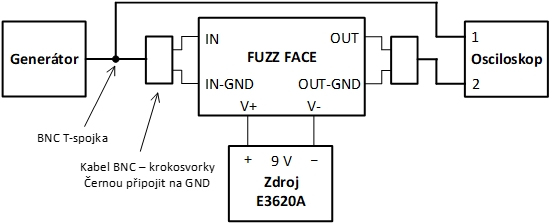
\includegraphics{ukoly_obrazek_1.png}
        % \caption{Zapojení diody v propustném a v závěrném směru}
    \end{figure}
    Napájecí napětí zdroje E3620A volte 9 V a využijte jeho příslušnou červenou a černou svorku. Zelenou svorku nezapojujte. Na osciloskopu nastavte synchronizaci (Trigger) pro nástupnou hranu výstupního signálu z obvodu (Source = 2). Pro lepší zobrazení malého vstupního signálu zvolte z nabídky Acquire průměrování zobrazení – Averaging pro 32 vzorků (\#Avgs = 32). Na generátoru nastavte sinusový průběh s kmitočtem 1 kHz a mezivrcholovou hodnotou 1 mVpp. Ve skutečnosti kvůli absenci 50 Ω zátěže bude hodnota výstupního napětí přibližně 2x vyšší. Je tedy vhodné při nastavování amplitudy na generátoru kontrolovat její skutečnou hodnotu osciloskopem. Pomocí měření mezivrcholové hodnoty osciloskopem (Meas, Type: Pk-Pk) tedy nastavte na generátoru mezivrcholovou hodnotu 2 mVpp, což odpovídá amplitudě 1 mV. Na generátoru by tomu mělo odpovídat nastavení amplitudy 1.1 mVpp. Pozor, na osciloskopu lze vybrat i měření „Type: Ampl“, to ale nezobrazuje amplitudu, ale opět mezivrcholovou hodnotu. Skutečná amplituda je tedy poloviční. Nezapomeňte aktivovat výstup generátoru pomocí stisku tlačítka Channel a volby Output On tlačítkem pod displejem. Průběhy vstupního a výstupního napětí z osciloskopu vložte do protokolu (např. uložením na USB flashdisk funkcí Save nebo vyfocením v dostatečné kvalitě). Opakujte totéž měření pro amplitudy vstupního napětí 5 mV a 20 mV – opět tyto hodnoty nastavujte podle osciloskopu. Získané průběhy vložte do protokolu, okomentujte a srovnejte s výsledky simulací z bodu 1).
    \item Zapojte obvod k externí zvukové kartě počítače M-AUDIO Fast Track a k osciloskopu podle následujícího obrázku.
    \begin{figure}[H]
        \centering
        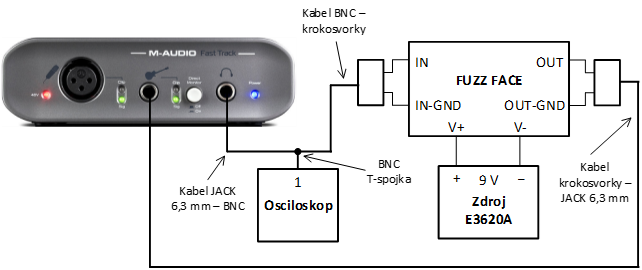
\includegraphics{ukoly_obrazek_2.png}
        % \caption{Zapojení diody v propustném a v závěrném směru}
    \end{figure}
    Jako vstup zvukové karty použijte zdířku JACK se symbolem kytary a jako výstup sluchátkovou zdířku JACK. Potenciometr Guitar Gain nastavte zhruba na polovinu rozsahu. Na počítači si překopírujte soubor \\ D:\textbackslash NKZT\textbackslash Audacity\textbackslash Fuzz\_face.aup3 do svého adresáře vytvořeného v D:\textbackslash student a poklikáním jej spusťte v programu Audacity. V souboru jsou připraveny dva zvukové signály – Test Tone a GTR. Stopa TestTone je harmonický testovací signál s kmitočtem 440 Hz a konstantní amplitudou. Tento signál slouží pro kalibraci úrovně výstupu zvukové karty. Klikněte na políčko „Solo“ pod názvem TestTone pro přehrávání pouze tohoto signálu. Na osciloskopu přepněte Acquire na „High Resolution“ a z nabídky „Meas“ zvolte typ zobrazení „AC RMS – Full Screen (Std Deviation)“. V Audacity spusťte přehrávání TestTone a pomocí ovládání hlasitosti potenciometrem Output na externí zvukové kartě nastavte úroveň výstupního signálu tak, aby byla hodnota AC RMS na osciloskopu 5 mV. Klikněte na tlačítko „Solo“ u druhé stopy s názvem GTR. Přesvědčte se, že na liště nad časovou osou programu je nastaveno „1 (Mono) Recording Channel“. Klikněte na připravenou prázdnou stopu s názvem 5mVrms, která bude mít zapnuté tlačítko „Mute“ a bude žlutě ohraničena. Stiskněte tlačítko „Skip to Start“, které se nachází napravo od tlačítka „Stop“. Spusťte nahrávání stiskem červeného tlačítka „Record“. Počkejte, až se přehraje a zaznamená celá zvuková stopa (cca 19 sekund) a poté stiskněte tlačítko „Stop“ pro ukončení nahrávání. Nahrávání podobně opakujte pro nastavení hodnoty RMS testovacího signálu na osciloskopu 20 mV a pro tento záznam využijte připravenou stopu s názvem 20mVrms. Pak si tyto nahrané stopy jednotlivě (se stiskem Solo) přehrajte a v protokolu zhodnoťte vliv efektu v závislosti na velikosti signálu. Dále porovnejte nahrané stopy se zvukovými výstupy z programu LTspice. Všechny vzniklé soubory je vhodné si uchovat pro zpracování protokolu.
\end{enumerate}

\section{Seznam použitých přístrojů}

\begin{enumerate}
    \item Generátor Agilent 33521A
    \item Zdroj Agilent E3620A
    \item Osciloskop Keysight DSO-X 2012A
    \item Externí zvuková karta M-Audio Fast Track
\end{enumerate}

\section{Zpracování úkolů}

\subsection{Úkol měření 1)}

% Popište, k jakým pozorovatelným jevům v obvodu dochází (zesílení, invertování signálů, zkreslení kladné, záporné, obou polarit signálů).

V této úloze jsme simulovali kytarový efekt Fuzz Face.
Na vstup byl přiveden sínusový signál o amplitudách 1 mV, 5 mV, 20 mV a 50 mV.
Na přiloženém obrázku níže jsou tyto jednotlivé signály vyobrazeny zelenou, modrou, červenou a tyrkysovou barvou.

Na spodním grafu (\textit{V(in)}) je možno vidět napěťové průběhy signálu na vstupu obvodu.
Na prostředním (\textit{V(col \_q1)}) jsou vyobrazeny napěťové průběhy z kolektoru tranzistoru Q1.
Nejvyšší graf (\textit{V(out)}) zobrazuje průběhy z výstupu obvodu.

\begin{figure}[H]
    \centering
    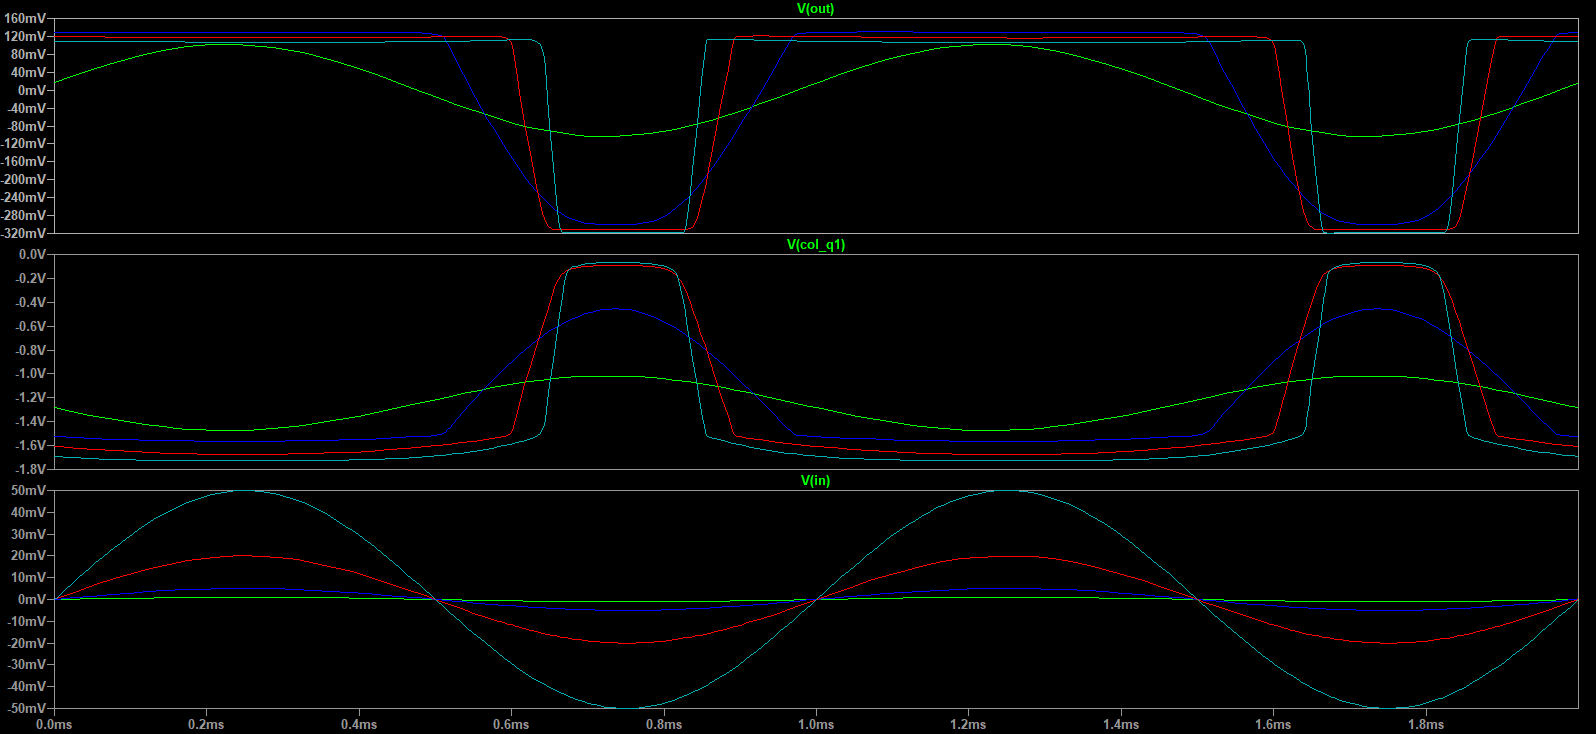
\includegraphics[width=\linewidth]{1_fuzz_face_trans.png}
    \caption{Simulace kytarového efektu Fuzz Face se sinusovým signálem na vstupu}
\end{figure}

Na průběhu z kolektoru tranzistoru Q1 pozorujeme, že dochází až k desetinásobnému zesílení vstupního signálu.
Signál je také výrazně posunut (má jinou střední hodnotu) a invertován.
U 1mV vstupního signálu, t.j. zeleného, pozorujeme desetinásobné zesílení, inverzi a stejnosměrné posunutí posunutí do záporu.
U modrého signálu pozorujeme kromě výše zmíněných jevů také "ořezání" spodní půlvlny.
Na signálech s vyšší amplitudou, t.j. červená a tyrkysová pozorujeme velmi výrazné nelineární zkreslení, kde dochází k ořezu i ve vrchní části signálu.

Na průbězích signálů na výstupu obvodu pozorujeme podobné jevy jako na kolektoru tranzistoru Q1.
Signál je však oproti předchozímu průběhu poměrně "stlačen" - je snížená dynamika.
Dále je signál opět invertován a posunut.
Vrchni třetina jeho rozsahu je nyní kladná, spodní dvě třetiny jsou záporné.
Tyto signály se stěží podobají původnímu signálu.
Jedná se spíše o obdélníkový (lichoběžníkový) signál, než sinusový.
Střída signálu je také výrazně jiná.

\subsection{Úkol měření 2)}

V tomto úkolu jsme se taktéž věnovali simulaci obvodu kytarového efektu Fuzz Face.
Tentokrát byl však na vstup obvodu přiveden zvukový soubor s kytarovou nahrávkou.

Na následujících dvou grafech jsou vyobrazeny napěťové průběhy signálů ze vstupu (zeleně) a výstupu (modře) obvodu.
Pro zřetelnost byl vybrán časový úsek nahrávky o délce 100 ms.
Na prvním grafu je vstupní signál zeslaben na efektivní hodnotu přibližně 5 mV.
Na druhém grafu je vstupní signál zeslaben na přibližně 20 mV.

\begin{figure}[H]
    \centering
    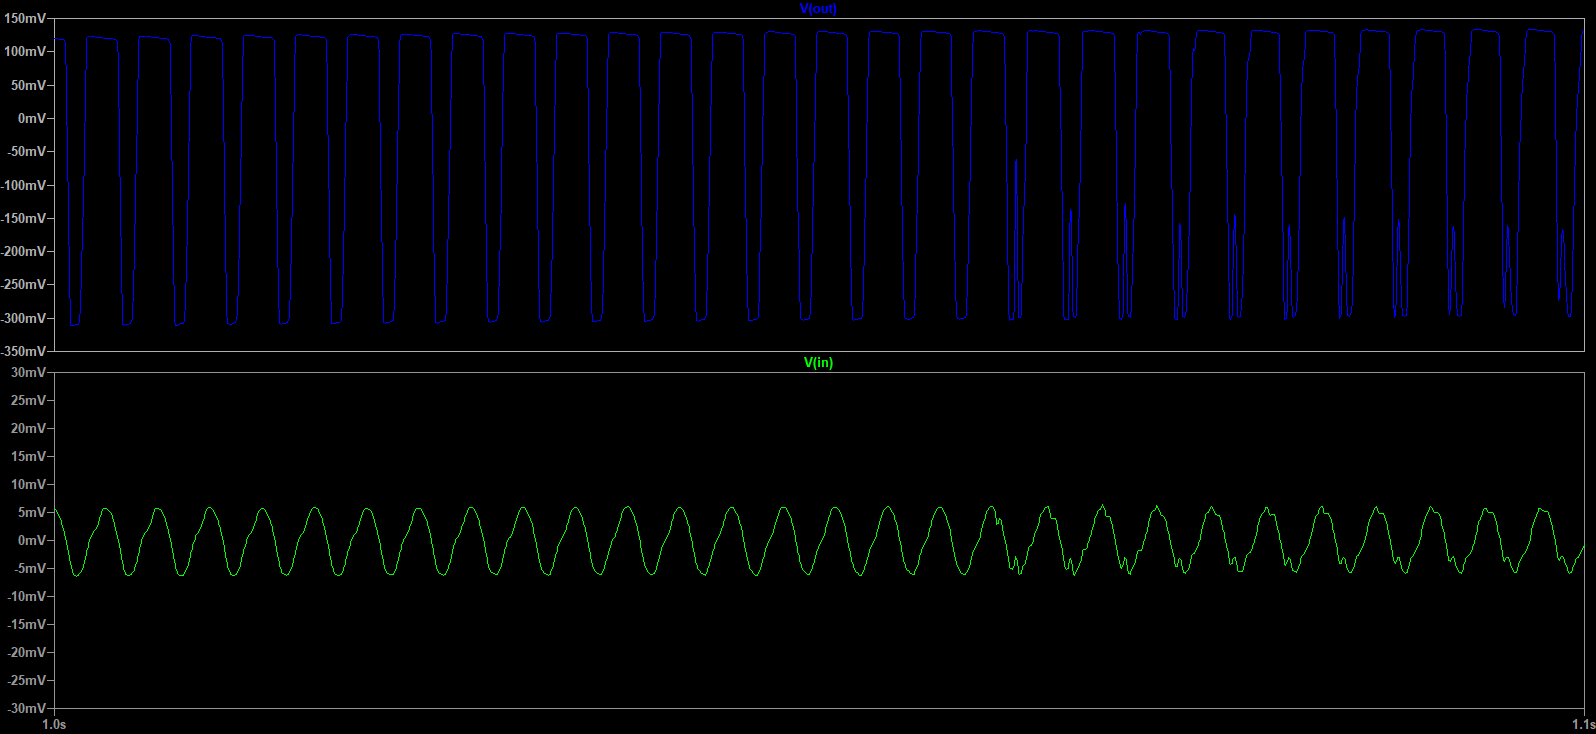
\includegraphics[width=\linewidth]{2_fuzz_face_zvuk_5mV.png}
    \caption{Simulace kytarového efektu Fuzz Face s kytarovou nahrávkou na vstupu - 5mV - konstanta 0,07}
\end{figure}

\begin{figure}[H]
    \centering
    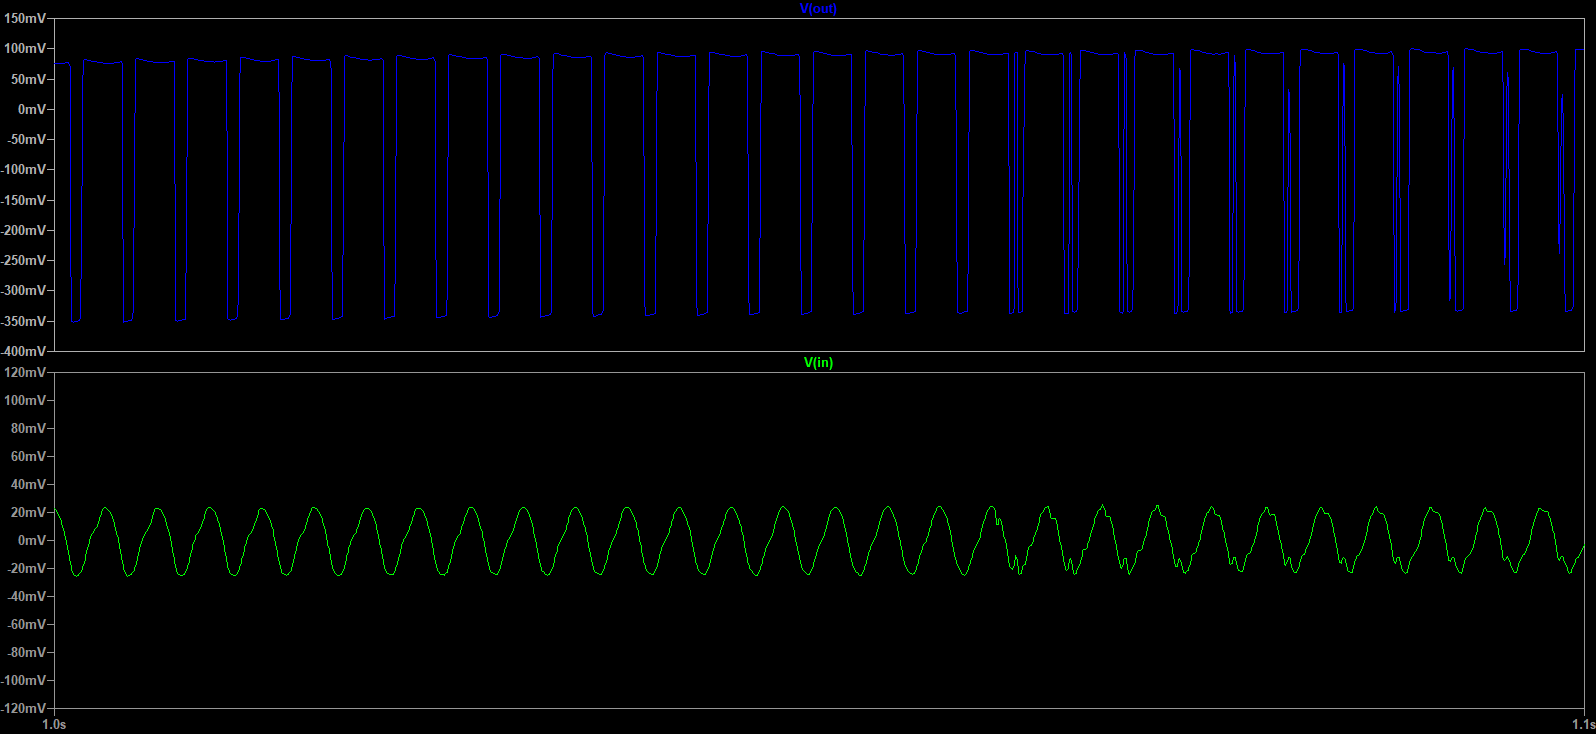
\includegraphics[width=\linewidth]{3_fuzz_face_zvuk_20mV.png}
    \caption{Simulace kytarového efektu Fuzz Face s kytarovou nahrávkou na vstupu - 20mV - konstanta 0,28}
\end{figure}

V této úloze pozorujeme podobné jevy jako v předcházející úloze - jednosměrné posunutí signálu do záporných hodnot, zkreslení a "ořezání" signálu.

Výstupní nahrávka ze simulace zní zkresleně a "špinavě", jako kdyby byl rozbitý kytarový zesilovač.
Druhá výstupní nahrávka z druhé simulace při 20 mV je velice zkreslená, zní až nepříjemně.

Vstupní nahrávka má délku cca. 5 sekund. Zpracování simulace však trvalo více než 12 sekund.
Délka simulace je nejspíše závislá na výpočetním výkonu použitého počítače.

\subsection{Úkol měření 3)}

V této úloze jsme se již věnovali měření na námi zkonstruovaném obvodu.
Na následujích obrázcích jsou zobrazeny kopie obrazovky laboratorního osciloskopu při různých amplitudách vstupního sinusového signálu - 1 mV , 5 mV a 20 mV.

\begin{figure}[H]
    \centering
    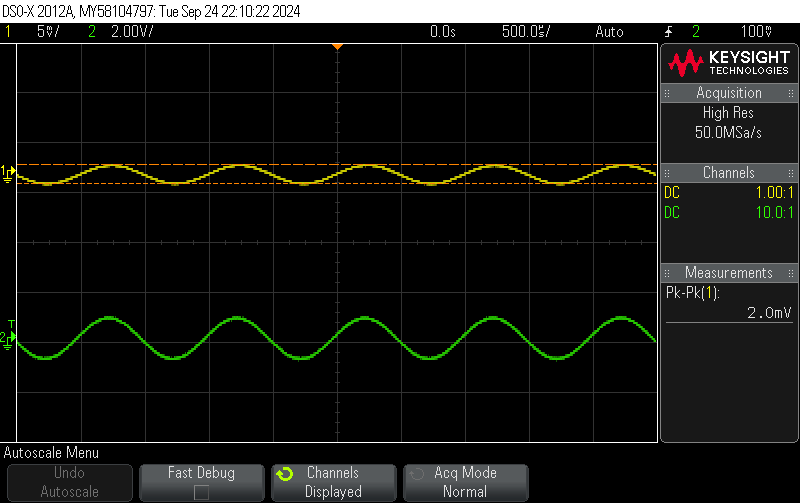
\includegraphics[width=\linewidth]{4_osciloskop.png}
    \caption{Kopie obrazovky z osciloskopu - sinusový signál s amplitudou 1 mV}
\end{figure}

\begin{figure}[H]
    \centering
    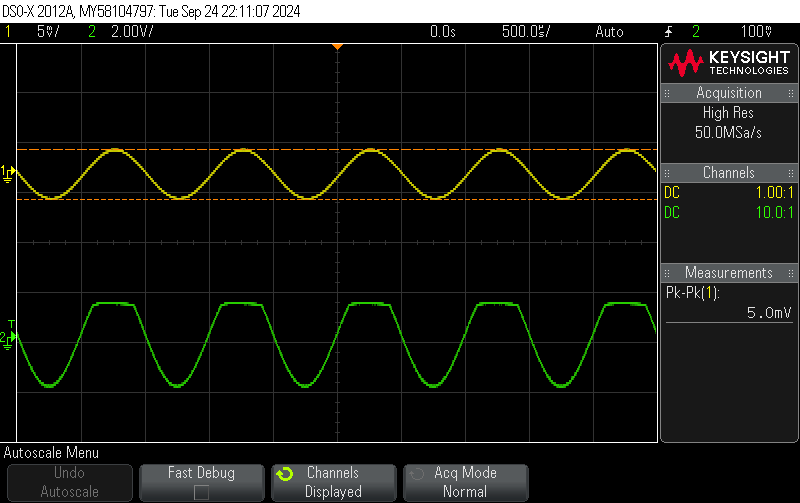
\includegraphics[width=\linewidth]{5_osciloskop.png}
    \caption{Kopie obrazovky z osciloskopu - sinusový signál s amplitudou 5 mV}
\end{figure}

\begin{figure}[H]
    \centering
    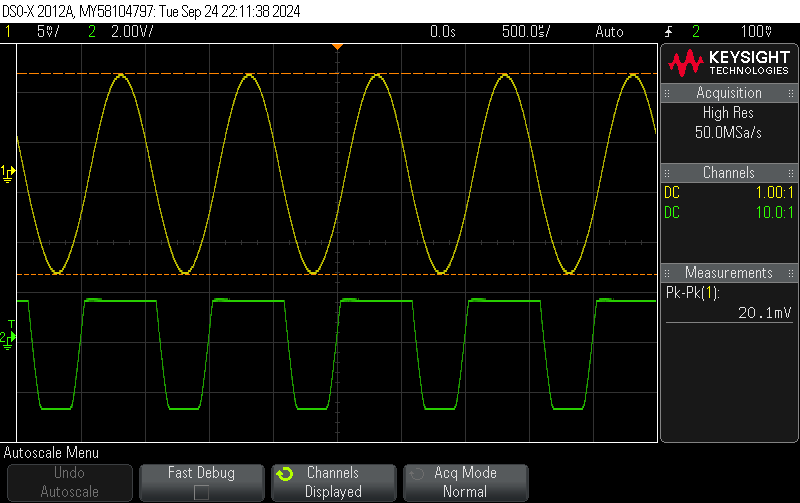
\includegraphics[width=\linewidth]{6_osciloskop.png}
    \caption{Kopie obrazovky z osciloskopu - sinusový signál s amplitudou 20 mV}
\end{figure}

Na těchto měřeních jsme pozorovali jevy prakticky totožené se simulací obvodu z úkolu 1) - jednosměrné posunutí signálu do záporných hodnot, zkreslení a "ořezání" signálu.
Je tedy patrné, že naše zkonstruované zapojení efektu Fuzz Face funguje správně. 

\subsection{Úkol měření 4)}

V této poslední úloze tohoto měření jsme se věnovali připojním zvukové kytarové nahrávky na vstup námi zkonstruovaného efektu pomocí externí zvukové karty M-Audio Fast track a počítačového programu Audacity.
Nejprve jsme funkčnost zapojení otestovali pomocí pomocí harmonického testovací signálu o frekvenci 440 Hz (komorní A).
Po ověření funkčnosti jsme se začali obvod zkoušet i s použitím dodané kytarové nahrávky.

Nejprve jsme měřili (nebo-li spíše poslechli) signál s hodnotou 5 mVrms, poté 20 mVrms.
Při poslechu bylo patrné, že obvod se ze zvukového hlediska chová velice podobně simulovanému obvodu z úkolu číslo 2).
Toto potvrzuje správnou funkčnost námi zkonstruovaného zapojení.
Výstupní nahrávka opět zní zkresleně a špinavě, no oproti simulovanému obovodu se nám (mně) zdá příjemnější na poslech.
To je zřejmé zejména u signálu s hodnotou 2O mVrms, který při simulaci zněl poměrně nepříjemně, zde však tak nepříjemný není.

\section{Závěr}

V tomto měření jsme se věnovali ve čtyřech úlohách simulaci a měření skutečného obvodu kytarového efektu Fuzz Face.
simulací jsme se se nejdříve seznámili se správným (předpokládaným) chováním obvodu.
Nabyté zkušenosti jsme poté využili při měření a zkoušení skutečného námi zkonstruovaného obvodu.

Během simulace jsme se seznámili se zajímavými jevy, kterých efekt Fuzz Face využívá - zejména zesílení, stejnosměrné posunutí. zkreslení a omezení dynamiky.
Zjistili jsme, že efekt Fuzz je v principu nesymetrickým omezovačem, který z vrchu omezuje dříve, než ze spodu (právě kvůli stejnosměrnému posunutí).
Výsledkem je tedy obdélníkový, nebo-li spíše lichoběžníkový signál, který je zkreslený a má střídu podstatnĚ jinou než původní signál.

Tento efekt by se dal popsat jako zkreslující, až "špinavý", při vyšších hodnotách může znít až nepříjemně.
Dal by se přirovnat ke zvuku rozbitého kytarového zesilovače.

\end{document}